
En las próximos secciones se hablará en mayor detalle del funcionamiento del programa implementado pero para los usuarios que quieran utilizar rápidamente nuestro software sin necesidad de entrar en detalles técnicos se describen a continuación los pasos a seguir para ejecutarlo.

\subsection{Requerimientos}

Para utilizar nuestro programa se necesita tener instalado Python 2.7 y C.
\\
\\
Las bibliotecas de Python utilizadas son las siguientes:

\begin{itemize}

\item cPickle
\item gzip
\item numpy
\item matplotlib
\item subprocess

\end{itemize}

\subsection{Preparación de datos de entrenamiento}

Una vez cumplidos los requerimientos se debe ejecutar el script de $Python$ ubicado en la carpeta $mnist$ en la raiz del proyecto. Este creará los archivos de entrenamiento que utilizará nuestro programa, los cuales están ubicados en la carpeta $data$.

\subsection{Ejecución del programa}

Con los archivos de entrenamiento listos ya podemos ejecutar el programa, este se ejecuta a partir de $program.py$ ubicado en la raiz del proyecto. Este programa recibe 3 parámetros, primero el lenguaje que queremos utilizar ($C$ o $asm$), luego el tipo de dato ($float$ o $double$) y por último la ubicación de la imagen del dígito que queremos predecir.
\\
\\
La imagen debe ser de 28x28 pixeles, como ejemplo está $test\_image.png$, para predecir el carácter escrito se utilizará entonces el siguiente comando.

\begin{verbatim}
                  python program.py asm float test_image.png
\end{verbatim}

Al ejecutar este comando se debería preparar la versión de red neuronal que tiene métodos implementados en $ASSEMBLER$ y que representa los valores de las matrices con floats.
\\
\\
Se debería recibir en la terminal algo similar a lo que se ve en la siguiente imagen.

\fboxsep=1mm%padding thickness
\fboxrule=2pt%border thickness

\begin{figure}[H]
\fcolorbox{black}{black}{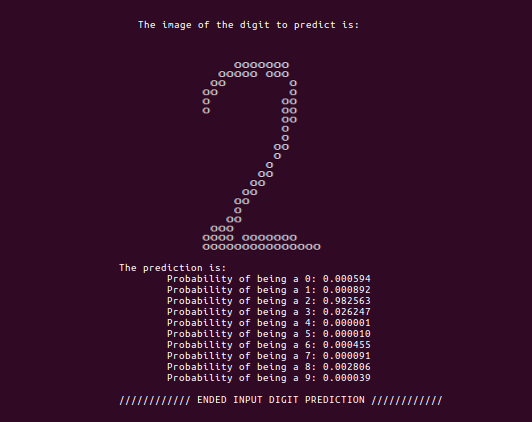
\includegraphics[scale=0.8]{imgs/example_execution.png}}
\centering
\caption{Imagen de ejemplo del output del programa}
\centering
\end{figure}